\section{Design and Implementation }

\subsection{Hardware ans Software}
This was run on a MacBook Pro computer using Iverilog. Additionally, gtkwave was used to monitor the wires.

\subsection{TSC design overview}

The TSC (Touch Sensing Controller) has a 3 bit state register, a 32-bit timer,
a 32-bit TRIGGER\_TM, and an internal ring buffer.
It is connected to the ADC (Analog-to-Digital Converter)
via a request (REQ), ready (RDY), and data (DAT) lines.
Additionally, the TSC can communicate with other devices using triggered (TRD), Send Buffer (SBF),
serial data (SD), and completed data (CD) registers and wires.


\begin{figure}[H]
    \centering
    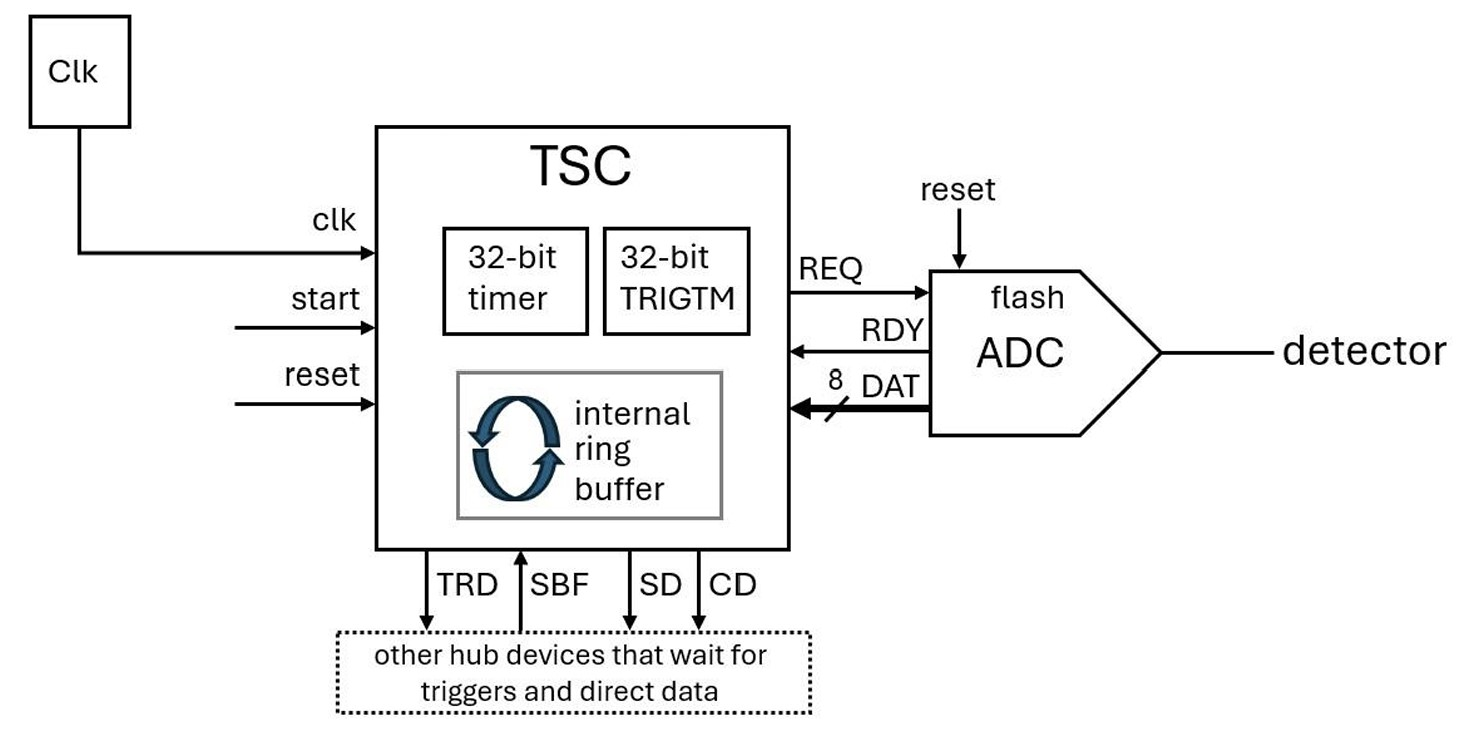
\includegraphics[width=0.8\columnwidth]{Figures/block_diagram_of_TSC}
    \caption{Block diagram of the TSC}
    \label{fig:block diagram of TSC}
\end{figure}

There is also an accompanying TSC\_tb test bench which is used to initiate and test the TSC module.

\subsection{CLock (clk)}
A 1 THz clock signal is set up on clk wire in the TS\_tb test bench.

\subsubsection{State register}
the st a register is a 3-bit register that has the folowing states:
\begin{itemize}
    \item 000 Stop :
          Initial state used to wait for reset pin has been triggered.
    \item 001 ready
          State that is enter on the reset pin rising edge and it waits for the start pin rising edge.
    \item 010 Running
          State that is entered from ready state once the start pin rising edge is pulled hight.
    \item 011 Triggered
          State entered when the value read by the ADC is
          greater than the predetermined trigger value (TRIGVL).
    \item 100 IDLE
          This state is entered when a trigger event has occurred
          and the TSC is waiting for the start pin or SPF pins rising edge.
    \item 101 SENDING
          This state is entered from the IDLE state when the SFB pin gos high. It indicates that data is being sent.
\end{itemize}


\subsubsection{Timer}
The timer is incremented on the rising edge of the clock. When
a trigger even occurs the timer si save in the TRIGTM register which is outputted to the test bench.
The timer is reset if a transition into a running state occurs.

\subsubsection{Ring Buffer}
The ring buffer is an array uf 32 8-bit register.
The tail pin index is named write_prt and is Initial set to \'b11111
and the tail index is named read_ptr and is initial set to 5\'b00000.
the head index is named head_ptr and is initial set to 5'b00000.
The 5 bit format for the head and tail index is used to iducate role offer at value 31.
and it store the values created by the ADC.

\subsubsection{how the TSC intervacec with the ADC}








